\documentclass[a4paper]{article}

\usepackage[utf8]{inputenc}
\usepackage[spanish]{babel}
\usepackage{float}
\usepackage{fancyhdr,graphicx,listings,amsmath,tocloft,color,soul}
\usepackage[colorlinks=true,linkcolor=black,urlcolor=blue,bookmarksopen=true]{hyperref}

\sethlcolor{red}

\newcommand{\materia}{[75.06 / 95.58] Organización de Datos}
\newcommand{\trabajo}{Trabajo Práctico 2: Machine Learning}
\newcommand{\trabajoheader}{TP2}
\newcommand{\cuatri}{2c2018}
\newcommand{\cuatrimestre}{Segundo cuatrimestre de 2018}
\newcommand{\grupo}{Grupo 30: Datatouille}
\newcommand{\repo}{https://github.com/FdelMazo/7506-Datos/}
\newcommand{\kernel}{https://kaggle.com/datatouille2018/}
\newcommand{\alumnos}{
    Bojman, Camila & 101055 &  camiboj@gmail.com\\
    del Mazo, Federico & 100029 & delmazofederico@gmail.com\\
    Hortas, Cecilia & 100687 & ceci.hortas@gmail.com\\
    Souto, Rodrigo & 97649 & rnsoutob@gmail.com\\
}
\newcommand{\curso}{Curso 01}
\newcommand{\docentes}{
    \item Argerich, Luis Argerich
    \item Golmar, Natalia
    \item Martinelli, Damina Ariel
    \item Ramos Mejia, Martín Gabriel
}

\hypersetup{
    pdftitle={\trabajo},
	pdfsubject={\materia},
	pdfauthor={\grupo},
}

\setlength{\cftbeforesecskip}{6pt}

\pagestyle{fancy}
\fancyhf{}
\fancyhead[L]{\materia}
\fancyhead[R]{\trabajoheader - \cuatri}
\renewcommand{\headrulewidth}{0.4pt}
\fancyfoot[C]{\thepage}
\renewcommand{\footrulewidth}{0.4pt}

\begin{document}
\pagenumbering{gobble}

\begin{titlepage}
	\hfill
\includegraphics[width=6cm]{fiuba.jpg}
    \begin{center}
    \vfill
    \Huge \textbf{\trabajo}
    \vskip2cm
    \Large \materia\\
    \cuatrimestre
    \vfill
    \begin{flushleft} 
    \grupo
    \end{flushleft}
    \begin{tabular}{|l|c|r|}
	\hline
	Alumno & Padrón & Mail\\
	\hline \hline
    \alumnos
	\hline
	\end{tabular}
    \begin{flushleft} 
    \large{\url{\repo}} \\
    \large{\url{\kernel}} \\
    \end{flushleft}
    \vskip1cm
    \end{center}
    \curso
    \begin{itemize}
        \docentes
    \end{itemize}
\end{titlepage}
\pagenumbering{roman}
\tableofcontents
\newpage
\pagenumbering{arabic}
\setcounter{page}{1}

\section{Introducción}

El objetivo principal del trabajo es predecir la probabilidad de que un usuario de la empresa Trocafone realice una compra (conversión) de un dispositivo celular. 

La realización del trabajo se hace con algoritmos de Machine Learning, una disciplina que busca poder generar clasificaciones en base a un entrenamiento sobre información pasada, seguida de una validación de las predicciones generadas. En el trabajo se prueban distintos algoritmos, los cuales todos en distinta manera hacen uso de los datos (en particular, de sus atributos). Es por esto que es muy importante saber qué datos usar, y buscar cómo codificarlos de tal forma que mejor se aprovechen.

Con dicho propósito se utilizan como base dos sets de datos brindados por la empresa. En un primer lugar el archivo \texttt{events\_up\_to\_01062018.csv} que contiene la información de los eventos realizados por un conjunto de usuarios desde el 1ro de enero hasta el 31 de mayo de 2018 y servirá como entrenamiento de los algoritmos, y en un segundo lugar el archivo \texttt{labels\_training\_set.csv} que determina si el usuario realizó o no una conversión desde el 1ro hasta el 15 de junio. Es este período es del cual se quieren predecir las conversiones. Siendo este segundo archivo un subconjunto del anterior, este servirá de validación de las predicciones.

\section{Organización del Trabajo}

Para un desarrollo más cómodo, se modularizó el trabajo en distintos notebooks de Jupyter que luego se importan entre sí\footnote{Haciendo uso del magnífico \href{https://github.com/grst/nbimporter}{nbimporter}}, intentando emular la programación estructurada. Si bien esta forma de trabajar sirve bastante para no estar repitiendo código, el dividir en distintos notebooks que dependan unos de otros sube el acoplamiento del proyecto en su totalidad.

Un pequeño índice del trabajo puede ser visto en \url{https://fdelmazo.github.io/7506-Datos/}.

Los notebooks, en orden de lectura y corrida son:

\begin{enumerate} 
	\item \textbf{Investigación Previa}

	\small{\url{https://fdelmazo.github.io/7506-Datos/TP2/investigacion.html}}

	En este notebook se presentan las distintas exploraciones que se hicieron sobre el dataset del trabajo práctico anterior (TP1\footnote{\url{{https://fdelmazo.github.io/7506-Datos/TP1/TP1.html}}})

	\item \textbf{Creación de dataframes}

	\small{\url{https://fdelmazo.github.io/7506-Datos/TP2/new_dataframes.html}}

	En este notebook se crean los distintos dataframes necesarios para poder extraer atributos de los usuarios.

	\item \textbf{Feature engineering}

	\small{\url{https://fdelmazo.github.io/7506-Datos/TP2/feature_engineering.html}}

	En este notebook se agregan todos los features que se consideran que pueden ser pertinentes para el modelo. Este notebook es el que genera el \texttt{user-features.csv} del cual entrenan los modelos.

	\item \textbf{Feature selection}

	\small{\url{https://fdelmazo.github.io/7506-Datos/TP2/feature_selection.html}}

	En este notebook se utilizan distintas formas de seleccionar los features con el objetivo de eliminar ruido y encontrar la mejor combinación de atributos a usar a la hora de entrenar modelos.

	\item \textbf{Parameter tuning}

	\small{\url{https://fdelmazo.github.io/7506-Datos/TP2/parameter_tuning.html}}

	En este notebook se hacen diversas pruebas sobre cada algoritmo hasta encontrar los híper-parámetros óptimos de cada uno.

	\item \textbf{Submission framework}

	\small{\url{https://fdelmazo.github.io/7506-Datos/TP2/submission_framework.html}}

	La principal idea de este notebook es definir una serie de pasos para armar las postulaciones de predicciones del trabajo práctico.

	\item \textbf{Notebook principal}

	\small{\url{https://fdelmazo.github.io/7506-Datos/TP2/TP2.html}}

	Finalmente, haciendo uso del framework previamente definido, se encuentra la combinación óptima de atributos y algoritmos para hacer una postulación de predicciones.

\end{enumerate}

\section{Features}
\subsection{Investigación previa}

El primer paso del trabajo consistió en realizar una investigación sobre lo ya hecho en el trabajo anterior. El TP1 es un análisis exploratorio de datos de la empresa. Si bien no son exactamente los mismos datos que los trabajados acá, son de la misma índole, y la exploración de ellos dan a luz a patrones en los usuarios del sitio.

Esta investigación se compone de dos partes, una técnica y otra teórica.

Por el lado técnico, viendo que se usó otro set de datos para el TP1, se buscó alguna forma de integrar los datos anteriores con los nuevos (por ejemplo, buscar si hay usuarios compartidos entre los dos sets, o si hay compras para registrar), para poder usar una base de datos más grande tanto para el entrenamiento como la validación de las predicciones. 

Luego de una serie de pasos, búsquedas y validaciones, se recopiló la siguiente información:
\begin{enumerate}
\item No se repiten usuarios en los datasets.
\item En el primer dataset (TP1) hay 27624 usuarios de los cuales 13967 tuvieron actividad en junio. Entre el 1 y el 15 (inclusive) de junio 82 usuarios compraron productos.
\item En el segundo dataset hay 19414 usuarios de los cuales 980 compraron en Junio.
\end{enumerate}

Se concluyó que hacer un merge de los datos del TP1 con los del TP2 presentaría un \textit{skewness} en el set de datos, por la despreciabilidad de estos.

Por otro lado, en un marco teórico, se vió el análisis hecho en búsqueda de qué patrones, ideas y conceptos pueden ser aplicados en este trabajo. En particular, se buscan atributos escondidos en el set original que puedan ser codificados de tal forma que luego los algoritmos de Machine Learning puedan utilizar a su favor. Los atributos encontrados son especificados en la sección de Feature Engineering.

Lo que se observó de analizar muchas muestras de usuarios que compraron, es ya sea en la sesión que efectuaron la compra, o en las anteriores, aumentaron considerablemente la cantidad de eventos, principalmente la vista de productos. Y en la recta final el comportamiento habitual es ver el mismo producto en varios de los colores disponibles.

\subsection{Clustering}

Con la intención de ver si se encontraban clusters que agrupen a los usuarios que compraron, se utilizó el algoritmo \texttt{T-SNE}, que es el estado del arte para la representación de datos en dos dimensiones.

\begin{figure}[!h]
	\makebox[\textwidth][c]{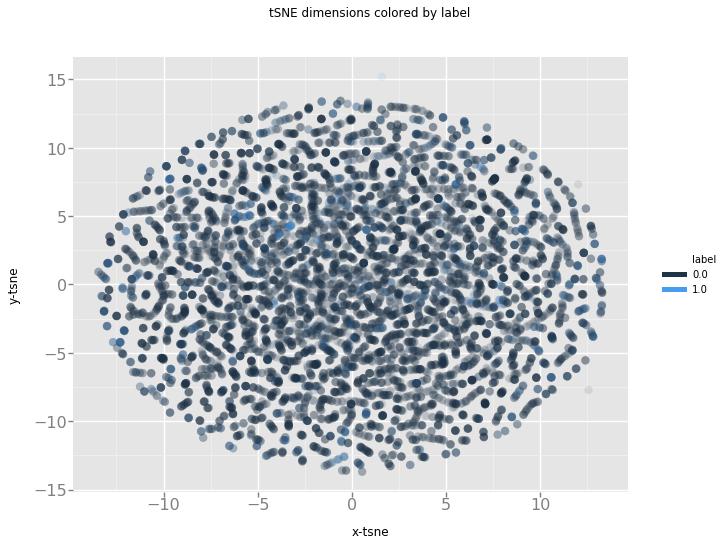
\includegraphics[width=0.8\textwidth]{figures/labels-2d.png}}
	\caption{Distribución usuarios que compraron}
	\label{fig:mesdiasnormalizado}
\end{figure}

\subsubsection{K-Means}

Decidimos utilizar este algoritmo debido a su simpleza y a que, según dicen, nunca funciona muy mal y a veces funciona muy bien.
Los resultados que se observan no son muy prometedores en vista a generar \textit{features}.

\begin{figure}[!h]
	\makebox[\textwidth][c]{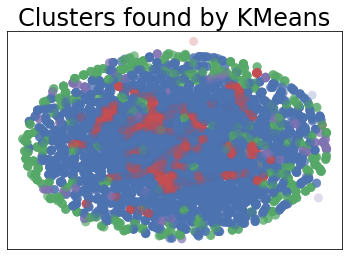
\includegraphics[width=0.8\textwidth]{figures/kmeans-4.png}}
	\caption{Clusters con K-Means. Cuatro clusters.}
	\label{fig:mesdiasnormalizado}
\end{figure}


\subsubsection{HDBScan}

Este algoritmo nos atrajo por ser el estado del arte en \textit{clustering}, pero a simple vista los resultados no parecen ser fructíferos, ya que genera una gran cantidad de \textit{clusters}, y no podemos aumentar mucho la cantidad mínima de elementos por cluster (híper-parámetro) debido a la naturaleza \textit{skewed} de los datos.

\begin{figure}[!h]
	\makebox[\textwidth][c]{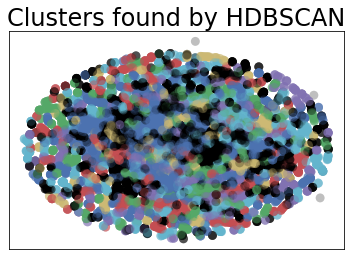
\includegraphics[width=0.8\textwidth]{figures/hdbscan-36.png}}
	\caption{Clusters con HDBScan. Min cluster size: 36.}
	\label{fig:mesdiasnormalizado}
\end{figure}



\subsection{Creación de dataframes}

Este es mayoritariamente un re-trabajo sobre lo hecho para el TP1, en el Notebook Anexo\footnote{\url{https://fdelmazo.github.io/7506-Datos/TP1/anexo.html}}.

Como parte del feature engineering, se crean dataframes nuevos con información de los productos del sitio y de cómo se accede a este. Los dataframes generados son:

\begin{itemize}
	\item \textbf{\texttt{brands.csv}}: Lista las marcas de los dispositivos de cada evento.
	\item \textbf{\texttt{os.csv}}: Lista los sistemas operativos desde los cuales se accedió al sitio.
	\item \textbf{\texttt{browsers.csv}}: Lista los exploradores desde los cuales se accedió al sitio.
	\item \textbf{\texttt{sessions.csv}}:  Se agregó el concepto de sesión, que se define como la agrupación de una serie de eventos por usuario, los cuales están todos con menos de 30 minutos de inactividad entre el actual y el anterior. 
	\item \textbf{\texttt{prices.csv}}: Lista los precios de los dispositivos de cada evento. Para lograr esto se hizo un \textit{web-scraping} de la página de Trocafone de la cual se extrajo para cada conjunto de modelo, capacidad, color y condición el precio del dispositivo.
\end{itemize}

\subsection{Feature engineering}

Con lo investigado del previó trabajo y todos los dataframes generados, se busca todo tipo de atributos de los usuarios, para que luego puedan ser seleccionados y aprovechados por los algoritmos a aplicar.

\subsubsection{Suma total de eventos}

\begin{sloppypar}
\texttt{\detokenize{['total_viewed_products', 'total_checkouts', 'total_conversions', 'total_events', 'total_sessions', 'total_session_checkout', 'total_session_conversion', 'total_events_ad_session', 'total_ad_sessions', 'avg_events_per_session', 'avg_events_per_ad_session', 'percentage_session_ad', 'percentage_session_conversion', 'has_checkout', 'has_conversion']
}}
\end{sloppypar}

Los atributos refieren a la sumatoria de cantidad de productos vistos, en checkout y en conversiones, más la totalidad de los eventos de cada usuario. Lo mismo para las sesiones de cada usuario y sus subtotales. También se agregan promedios de eventos por sesión y porcentajes de los accesos de las sesiones del usuario.

\subsubsection{Cantidad de eventos por mes}

\begin{sloppypar}
\texttt{\small{\detokenize{['total_viewed_products_month_1', 'total_checkouts_month_1', 'total_conversions_month_1', 'total_events_month_1', 'total_sessions_month_1', 'total_session_checkouts_month_1', 'total_session_conversions_month_1', 'total_events_ad_session_month_1', 'total_ad_sessions_month_1', 'has_checkout_month_1', 'has_conversion_month_1', 'total_viewed_products_month_2', 'total_checkouts_month_2', 'total_conversions_month_2', 'total_events_month_2', 'total_sessions_month_2', 'total_session_checkouts_month_2', 'total_session_conversions_month_2', 'total_events_ad_session_month_2', 'total_ad_sessions_month_2', 'has_checkout_month_2', 'has_conversion_month_2', 'total_viewed_products_month_3', 'total_checkouts_month_3', 'total_conversions_month_3', 'total_events_month_3', 'total_sessions_month_3', 'total_session_checkouts_month_3', 'total_session_conversions_month_3', 'total_events_ad_session_month_3', 'total_ad_sessions_month_3', 'has_checkout_month_3', 'has_conversion_month_3', 'total_viewed_products_month_4', 'total_checkouts_month_4', 'total_conversions_month_4', 'total_events_month_4', 'total_sessions_month_4', 'total_session_checkouts_month_4', 'total_session_conversions_month_4', 'total_events_ad_session_month_4', 'total_ad_sessions_month_4', 'has_checkout_month_4', 'has_conversion_month_4', 'total_viewed_products_month_5', 'total_checkouts_month_5', 'total_conversions_month_5', 'total_events_month_5', 'total_sessions_month_5', 'total_session_checkouts_month_5', 'total_session_conversions_month_5', 'total_events_ad_session_month_5', 'total_ad_sessions_month_5', 'has_checkout_month_5', 'has_conversion_month_5']
}}}
\end{sloppypar}

Se codifican la cantidad de productos vistos por mes por usuario, los productos en checkout, en conversion, las sesiones, y demás.

\subsubsection{Eventos sin contar mayo}

\begin{sloppypar}
	\texttt{\small{\detokenize{['total_viewed_products_months_1_to_4', 'total_checkouts_months_1_to_4', 'total_conversions_months_1_to_4', 'total_events_months_1_to_4', 'total_sessions_months_1_to_4', 'total_session_checkouts_months_1_to_4', 'total_session_conversions_months_1_to_4', 'total_events_ad_session_months_1_to_4', 'total_ad_sessions_months_1_to_4', 'has_checkout_months_1_to_4', 'has_conversion_months_1_to_4']
	}}}
\end{sloppypar}

La idea de esta funcionalidad es contar la cantidad de checkouts y conversiones por usuario excluyendo a mayo. Luego de hacer este feature notamos una mejora en el rendimiento de las predicciones por lo cual se lo mantuvo.


\subsubsection{Eventos en última semana}

\begin{sloppypar}
	\texttt{\small{\detokenize{
		['total_viewed_products_last_week', 'total_checkouts_last_week', 'total_conversions_last_week', 'total_events_last_week', 'total_sessions_last_week', 'total_session_checkouts_last_week', 'total_session_conversions_last_week', 'total_events_ad_session_last_week', 'total_ad_sessions_last_week', 'has_checkout_last_week', 'has_conversion_last_week']
	}}}
\end{sloppypar}

Aquí la idea pensada es reflejar la cantidad de eventos del usuario de la última semana. La principal idea radica en estimar que si el usuario ingresó muchas veces a la página en la última semana de mayo es muy probable que compre en la primera semana de junio. De la misma manera, también podría considerarse que si el usuario compró la última semana de mayo es probable que no compre por las siguientes dos.

\subsubsection{Distribución mensual de las conversiones}

\begin{sloppypar}
	\texttt{\detokenize{
		['amount_of_months_that_has_bought']
	}}
\end{sloppypar}

Se agrega en cuántos meses el usuario compró suponiendo que dicha distribución denota si el usuario es un comprador habitual o sólo compró alguna vez aisladamente. 

\subsubsection{Informacion de los últimos eventos registrados por usuario}

\begin{sloppypar}
	\texttt{\detokenize{
		['timestamp_last_event', 'timestamp_last_checkout', 'timestamp_last_conversion', 'timestamp_last_viewed_product', 'days_to_last_event', 'days_to_last_checkout', 'days_to_last_conversion', 'days_to_last_viewed_product', 'doy_last_event', 'dow_last_event', 'dom_last_event', 'woy_last_event', 'doy_last_checkout', 'dow_last_checkout', 'dom_last_checkout', 'woy_last_checkout', 'doy_last_conversion', 'dow_last_conversion', 'dom_last_conversion', 'woy_last_conversion', 'doy_last_viewed_product', 'dow_last_viewed_product', 'dom_last_viewed_product', 'woy_last_viewed_product']
	}}
\end{sloppypar}

Se busca extraer información de los días que transcurrieron hasta el último evento de un usuario. De esta manera se espera que el modelo aprenda un factor importante para la predicción. Por ejemplo, si un usuario vió un producto hace muchos días es muy probable que no lo compre pero si hizo checkout hace 1 dia es probable que en un futuro cercano compre.
	
En paralelo con estos features se consideran los días de la semana, del mes, del año y la semana del año donde ocurren estos últimos eventos.	
	
\subsubsection{Precios de la ultima conversion realizada por el usuario}

\begin{sloppypar}
	\texttt{\detokenize{
		['last_conversion_sku', 'last_conversion_price']
	}}
\end{sloppypar}

Se especuló que podría considerarse el precio de la última conversión del usuario como un feature pero a la hora de la selección reflejó una importancia muy baja. Por lo tanto consideramos impertinente la descripción de la idea que habíamos pensado desarrollar.

\subsubsection{Porcentaje de la actividad de la ultima semana}

\begin{sloppypar}
	\texttt{\small{\detokenize{
		['percentage_last_week_activity', 'percentage_last_week_conversions', 'percentage_last_week_checkouts', 'percentage_last_week_viewed_products']
	}}}
\end{sloppypar}

La intención en este feature es terminar de cerrar un tema que queda inconcluso en el feature ’Eventos en última semana’. Es verdad que si un usuario e en el último tiempo viene visitando mucho la página, sin comprar, es más probable que compre que otro que no. Por otro lado, existen usuarios que previó
a comprar hacen pocas visitas y no se los estaría teniendo en cuenta.

En conclusión, con el porcentaje se busca analizar si el usuario comenzó a generar más eventos de lo regular . Es decir, si el cliente modificó su conducta habitual. Entonces para ello se cacula la cantidad de eventos del usuario de la última semana sobre el total.

\subsubsection{Porcentaje de la actividad del ultimo mes}

\begin{sloppypar}
	\texttt{\small{\detokenize{
		['percentage_last_month_activity', 'percentage_last_month_conversions',
		 'percentage_last_month_checkouts', 'percentage_last_month_viewed_products']
	}}}
\end{sloppypar}

Una lógica análoga a la sección precedente se sigue en esta parte. Los motivos de este feature son simplemente una ampliación de la idea anterior. Si el usuario ingresó más de lo habitual a la página en mayo es muy probable que compre en la primera semana de junio. De la misma manera, si el usuario compró en mayo, no siendo este su comportamiento regular, es algo probable que no compre por las siguientes dos.

\subsubsection{Días entre el último checkout y última actividad}

\begin{sloppypar}
	\texttt{\detokenize{
		['days_between_last_event_and_checkout']
	}}
\end{sloppypar}

La intención de este feature es medir la diferencia de días que tiene cada usuario entre la compra de un celular y la ultima vez que visualizo el producto comprado. De esta forma se espera poder predecir en base a los productos vistos si es posible que el usuario efectúe una compra.

\subsubsection{Estados de celulares}

\begin{sloppypar}
	\texttt{\detokenize{
		['percentage_regular_celphones_activity']
	}}
\end{sloppypar}

Utilizando la lógica de que hay empresas que compran celulares en mal estado con el único fin de usar sus partes como respuestos se plantea agregar una columna que indique porcentaje de celulares en estado Bom - Sem Touch ID vs Bom sobre todos los celulares vistos.

\subsubsection{Varianza logarítmica de productos vistos}

\begin{sloppypar}
	\texttt{\detokenize{
		['var_viewed']
	}}
\end{sloppypar}

Se propone analizar la varianza en los precios de los productos visitados. Es decir, si los usuarios ven telefonos de un rango pequeño de precio o, por el contrario, articulos de precios muy variados. Se utilizó una escala logarítmica para seguir manteniendo las proporciones sin tener una gran diferencia entre la varianza de un usuario y la de otro.

\subsubsection{¿El usuario compró más de la media?}

\begin{sloppypar}
	\texttt{\detokenize{
		['conversion_gt_media']
	}}
\end{sloppypar}

Se propone como feature evaluar si el usuario compró un celular por encima de la media de precios. 

\subsubsection{¿Cuántas veces vió el último modelo que compró?}

\begin{sloppypar}
	\texttt{\detokenize{
		['total_max_viewed_product','percentage_max_viewed_product']
	}}
\end{sloppypar}

La idea de este atributo es evaluar una cierta correlación entre los usuarios de la cantidad de veces que se ve un modelo antes de comprarlo. Si un usuario ve una cantidad significativamente grande de veces un modelo es muy probable que lo compre. Esto no quiere decir que sea imposible que un usuario pueda ver una vez un modelo y no comprarlo o verlo muchas veces y no comprarlo pero se busca analizar el caso más general.

\subsubsection{¿Cuántas veces vió la última marca que compró?}

\begin{sloppypar}
	\texttt{\detokenize{
		['cant_viewed_brand_last_conversion']
	}}
\end{sloppypar}

Una lógica similar a la sección precedente es la que se sigue con este feature. La idea sería también analizar si un usuario se restringe a un modelo en particular o si puede ver distintos celulares de la misma marca y elegir uno de ellos.

\subsubsection{Comportamiento en sesiones de las últimas semanas}

\begin{sloppypar}
	\texttt{\detokenize{
		['ratio_sessions_last_week_over_total', 'has_event_last_week']
	}}
\end{sloppypar}

Se presenta una idea similar a la de las secciones \texttt{3.9} y \texttt{3.10}:

\subsubsection{¿Cuántas veces entró cada usuario a las static pages?}

\begin{sloppypar}
	\texttt{\detokenize{
	['cant_visitas_customer_service', 'cant_visitas_faq_ecommerce']
	}}
\end{sloppypar}

Considerando la poca fama de las secciones de ”preguntas frecuentes" se pensó que podía exixtir una relación directa entre el compromiso del cliente con la compra/estudio de mercado y la visita a las mismas. Dado que la cantidad de eventos para la mayoría de las static pages son despreciables se tomaron las dos más frecuentes ’FaqEcommerce’ y ’CustomerService’.

\subsubsection{¿Cuántas veces vió el modelo que más vió la última semana?}

\begin{sloppypar}
	\texttt{\small{\detokenize{
	['total_last_week_viewed_products', 'total_last_week_max_viewed_product', 'percentage_last_week_max_viewed_product']
	}}}
\end{sloppypar}

Nos parece evidente que existe una correlación entre ver mucho un articulo o modelo y el deseo de comprarlo. Por lo tanto en esta funcionalidad propone analizar cuántas veces el usuario vió alguna publicación del modelo con mayor probabilidad de compra (el que más visitó) indiferentemente de cuál sea este modelo. 

Se propone también analizar esta información para un rango de tiempo no muy extenso y cercano (en función a la fecha) a los labels que se quieren predecir. 

\subsubsection{Valores de clusters}

\begin{sloppypar}
	\texttt{\detokenize{
	['kmeans_3', 
	'kmeans_5',
	'kmeans_6',
	'kmeans_15',
	'kmeans_25,
	'hdbscan_22',
	]
	}}
\end{sloppypar}

A modo de prueba, decidimos crear features que tengan como valor el número de \textit{cluster} que le dio el algoritmo usado.

\subsubsection{Marca más vista}

\begin{sloppypar}
	\texttt{\detokenize{
	[
'most_viewed_brand_is_asus', 	'most_viewed_brand_is_ipad', 	'most_viewed_brand_is_iphone', 	'most_viewed_brand_is_lenovo', 	'most_viewed_brand_is_lg', 	'most_viewed_brand_is_motorola',	'most_viewed_brand_is_quantum', 	'most_viewed_brand_is_samsung', 	'most_viewed_brand_is_sony'	]
	}}
\end{sloppypar}

Se realizó \texttt{One Hot Encoding} para obtener cuál fue la marca más vista por el usuario, tanto en el total del período como en la última semana.

\subsection{Feature selection}

Una vez que se tienen todos los atributos en un mismo dataframe y luego de un par de pruebas se ve que no siempre hay que entrenar los modelos con la totalidad del dataframe. Viendo que para algunos algoritmos el orden y la selección de los features logrababa distintos resultados, se busca la forma de encontrar la combinación óptima de features y eliminar todo el ruido posible.

El modelo usado de referencia para esta sección es el de Random Forest debido a su estabilidad para mostrar la importancia de cada feature. Su funcionamiento radica en que los árboles que crea el algoritmo toman distintos subconjuntos de atributos tomados al azar y arrojan distintos resultados. De esta manera, con cientos o miles de árboles el algoritmo adopta una amplia capacidad predictora de cada atributo.

Es importante notar que a mayor cantidad de árboles generados por Random Forest, más precisa será la importancia del feature, ya que más árboles al azar tendrán los features y mejor se podrá estimar cuánto aportaron en cada árbol. Esto, en cuanto al modelaje para la predicción no es tan importante, ya que eventualmente el retorno de las ganancias será despreciable, pero para lo que es importancia de atributos es fundamental.

Se utiliza como métrica el area bajo la curva debido a que es la utilizada por la plataforma de Kaggle para evaluar la eficiencia de los distintos modelos utilizados. 

Siendo este el proceso más costoso de todo el trabajo, al ver que cada método puede llegar a tener que evaluar modelos que ya fueron probados previamente, en un intento de \textit{programación dinámica} se van guardando todos los resultados corridos para poder acceder a ellos sin tener que hacer una ejecución que ya fue hecha.

Las distintas formas de selección utilizadas son:

\begin {itemize}

\item \textbf{Métodos greedy}

\begin {itemize}

	\item \textbf{Cumulative Importance}

	Este método es el más intuitivo para la selección de features debido a su naturaleza \textit{greedy}. La idea es primero correr el Random Forest sobre todo el dataframe, y sobre este resultado obtener la importancia de cada feature. Ahora, con los features ordenados según importancia se genera una lista de listas que agrega un feature a la vez. Por ejemplo siendo \texttt{a,b,c} los features ordenados, se obtienen las listas \texttt{a}, \texttt{a,b} y  \texttt{a,b,c}.

	Ahora, con la lista de listas de features según importancia, se corre un Random Forest para cada subconjunto, en busqueda del \textit{codo}, es decir, el subconjunto que mayor AUC tenga antes de decaer a los features ruidosos.

	La desventaja que presenta este método es que parte del supuesto de que la importancia de cada feature es la misma para la corrida del dataframe entero que para subconjuntos de esto, lo cual no es cierto. De todas formas, es uno de los métodos que mejores resultados dió.

\end{itemize}

\item \textbf{Métodos de fuerza bruta}

\begin{itemize}

	\item \textbf{Forward Selection}

	Con este método se comienza con ningún atributo y en cada paso se agrega el atributo que genere mejor resultado. Se agregan atributos siempre y cuando los resultados mejoren. El algoritmo termina cuando el resultado no se puede mejorar o cuando ya se han agregado todos los atributos.

	\item \textbf{Backward Elimination}

	Este método funciona a la inversa de Forward Selection. Se comienza con todos los atributos y se quita en cada iteración el atributo que menos aportaba. De esta manera el algoritmo termina cuando al quitar un atributo el resultado empeora o cuando ya no hay más atributos por quitar.

	\item \textbf{Stepwise Selection}

	Este método es una combinación de ambos métodos descritos anteriormente. La idea es partir de una lista vacía como en Forward Selection, y agregar siempre el mejor atributo posible (como Forward Selection). Luego, una vez que se tiene el mejor atributo, se busca recursivamente con Backward Elimination si algún atributo sobra. Es una forma sabia de moverse a traves de los atributos; en cada paso se agrega el mejor posible y saca todos los que empeoraban esa nueva combinación.

\end{itemize}

El mayor problema de estos tres métodos es que, si bien son efectivos en los subconjuntos encontrados, son muy costosos en tiempo (como todo algoritmo de fuerza bruta). Pensar que se hacen \texttt{n} iteraciones (siendo \texttt{n} la cantidad de features) y para cada una de esas iteraciones se hacen \texttt{n} más (y ni pensar en Stepwise Selection, que hace aún \texttt{n} más). Pasados los 100 features ya esto pasa a ser increiblemente costoso. Es por esto que se le agrega una condición de corte, donde si para las x iteraciones no se encuentra una mejora simplemente se corte el proceso. Si bien esto plantea la posibilidad de caer en un máximo local, en tiempo termina siendo rendidor.

\item \textbf{Métodos de otras heurísticas}

Se agregan algunos criterios más, para aumentar los subconjuntos a utilizar.

\begin{itemize}

	\item \textbf{Full Dataframe} Como su nombre lo dice, simplemente probar el modelo sobre el dataframe entero.

	\item \textbf{Selección a Mano} Para no confiar solamente en los métodos algorítmicos, se hacen selecciones de los features manualmente.

	\item \textbf{Random Selection} También se hacen selecciones azarosas de \texttt{n} atributos, para así en cada corrida ver si se encuentra alguna buena combinación que sirva para la selección manual o de una idea de qué atributos ayudan o no.

	\item \textbf{Feature Intersection} Aprovechando que se tienen muchas formas distintas de seleccionar subconjuntos, también se utiliza como método el intersectar todas estas combinaciones, con la idea de que si un feature aparece en varios de los subconjuntos anteriores, pues ciertamente será bueno por si mismo.

\end{itemize}														

\end {itemize}


\section{Modelos}

\subsection{Algoritmos de clasificación utilizados}

\subsubsection{Árboles de decisión}

Este algoritmo se constituye de un árbol binario cuyos niveles se dividen en dos a partir del set de datos. Finalmente, es en los nodos hoja donde se clasifican los datos.

Este modelo trajo grandes resultados usado por sí solo y es uno de los algoritmos que más fueron postulados.

\subsubsection{Random forests}

Se constituye de un ensamble de árboles de decisiones con subconjuntos de los atributos a utilizar, y con la técnica de \textit{bagging} se selecciona finalmente el promedio de los árboles corridos.

Este modelo tan popular trajo buenos resultados, pero bastante a la par con los de árboles de decisiones (se pretendía que sea ampliamente mejor). Una gran ventaja de este modelo es evitar el overfitting, por lo cual es de los modelos más confiables del trabajo. 

Es esta resistencia al overfitting y que siempre usa subconjuntos en cada árbol lo que lo hacen el algoritmo más estable para ver la importancia de cada atributo, como ya se marcó en la sección de \textbf{Feature Selection}.

Sus dos híper-parámetros son la cantidad de árboles a utilizar y la cantidad de atributos por árbol. Otra característica de este modelo es su invariante frente a la escala de los atributos, es decir, no hay que normalizar los datos.

\subsubsection{XGBoost}

XGBoost es un algoritmo muy eficiente de gradient boosting en árboles. Uno de sus híper-parámetros más importantes es la funcion objetivo, de la cual se usa la logística binaria, ya que se tiene un problema de clasificación binaria y no uno de regresión.

Este algoritmo nos dio los mejores resultados hasta ser reemplazado por LightGBM.

La gran cantidad de híper-parámetros que tiene nos llevó a usar una búsqueda aleatoria de estos con cross validation, de lo cual se hablará más adelante.

\subsubsection{KNN}

Un algoritmo sencillo utilizado es el de los K vecinos más cercanos. Este algoritmo consiste en encontrar los vecinos más cercanos del punto a clasificar, y luego simplemente predecir que el punto en cuestión es de la clase del cual la mayoría de sus vecinos sean parte. Sus híper-parámetros a definir es la cantidad de vecinos a tomar en cuenta y la distancia a utilizar entre ellos. 

Es tal vez en su sencillez que está una de sus mayores desventajas: es un algoritmo de orden cuadrático, y esto impacta mucho sobre la ejecución de cada modelo que se hace. Otra cosa a remarcar es que los datos deben estár normalizados a la hora de procesarlos.

Si bien es un algoritmo muy sencillo y básico de Machine Learning, también es uno que, con sus híper-parámetros bien configurados, mejores resultados da. 

\subsubsection{Naïve-Bayes}

Este algoritmo, basado en el teorema de Bayes, es sencillo y bastante rápido. No suele tener los mejores resultados, pero era un algoritmo básico a probar. Su inocencia proviene del iluso supuesto de que las dimensiones son independientes entre sí, pero no por esto deja de ser un buen clasificador.

Si bien no dio siempre los mejores resultados, si se notó su rapidez y su facilidad para tratar con la gran dimensión de los datos.

El algoritmo fue utilizado en todas sus variantes (que conocemos):


\begin{itemize}
	\item \textbf{Gausiano}
	
	\item \textbf{Bernouilli}
	
	\item \textbf{Multinomial}	
	
 	\item \textbf{Complemento}
\end{itemize}


\subsubsection{Redes neuronales}

Un algoritmo utilizado para buscar alguna aproximación no lineal fue el de redes neuronales. Algo que no hay que olvidar es de normalizar los datos (no hacerlo da la sensación de que el algoritmo es mucho peor de lo que verdaderamente es, ya que esto es algo fundamental de las redes). 

Este algoritmo no dio tan buenos resultados para la cantidad de tiempo que consume.

\subsubsection{LightGBM}

LightGBM es simplemente el algoritmo que constantemente mejores resultados nos dió. Este algoritmo de gradient boosting sobre árboles se diferencia de XGBoost en que construye los árboles según las hojas, y no los niveles. Es importante que sus híper-parámetros estén bien configurados (por ejemplo, la profundidad máxima de los árboles), y es aquí donde se notó el mayor incremento en el AUC, un LightGBM con sus híper-parámetros no tan cuidados da resultados tan malos que ni se ocurre usarlo de nuevo, y es recién cuando uno se pone a hilar fino entre los parámetros (y sale de los de defecto) que rápidamente se encuentran muy buenos saltos de calidad en el modelo.

Este algoritmo también se destaca por ser rápido y consumir poca memoria. También, tiene un gran manejo de la dimensionalidad de los datos, sin cambiar mucho frente a ellos.

\subsubsection{Gradient boosting}

Viendo los resultados que XGBoost y LightGBM daban, se opto por usar el clasificador base de gradient boosting, que si bien dio resultados favorables, no llega a superar a los modelos previamente utilizados.

\subsubsection{Catboost}

Despues de probar gradient boosting, optamos por usar más modelos de esa indole. Catboost es el último algoritmo de boosting probado y sus resultados no fueron tan buenos como para justificar el tiempo perdido en cada ejecucion. Es fácilmente el modelo más lento de todo lo corrido.

\subsubsection{Adaboosting}

En este caso seguimos manejando modelos de la familia de boosting. 

Adaboosting comienza con un clasificador simple que va siendo modificado dependiendo su nivel de error. En cada iteración se le da peso a la clase que mejor resultado obtuvo y luego se vuelve a iterar. 

Una vez finalizadas las iteraciones se crea un promedio ponderado. Esta combinación lineal de los N clasificadores va a ser su clasificador final.

\subsection{Parameter tuning}

En los primeros modelos corridos fue cuando se empezo a notar lo que ya se sabía: los híper-parámetros son sencillamente lo más importante de cada algoritmo, y la diferencia entre un buen modelo y uno promedio o incluso malo.

Inicialmente, debido a la gran cantidad de opciones para algunos algoritmos, optamos por un método greedy, que consistía en un pequeño framework donde se van probando distintos híper-parámetros con distintos valores progresivamente. Es decir, se parte un grid search grande en varios más pequeños, ya que por la naturaleza del algoritmo este proceso es muy costoso en tiempo. Si bien esto no encuentra la combinación óptima, al menos da resultados bastante favorables y se ahorra mucho tiempo de ejecución.

Esto dio resultados cuestionables, por lo que implementamos una búsqueda aleatoria de híper-parámetros, y luego, utilizamos grid search (un método de fuerza bruta que lo que hace es correr las posibilidades planteadas hasta encontrar la mejor combinación de los híper-parámetros a probar) sobre un rango acotado basado en los resultados anteriores.

Las herramientas que utilizamos para esto nos permitían elegir la métrica a maximizar, y usamos AUC ROC.

\subsection{Ensambles}

\subsubsection{Bagging}

El bagging consiste en aplicar un clasificador n veces y luego promediar el resultado final. Es importante que cada una de las corridas del clasificador sea con datos reemplazados en el set de entrenamiento (\textit{bootstrapping}).

La principal ventaja generada es evitar el overfitting, ya que ningún clasificador conoce el set de entrenamiento completo y por lo tanto no se puede sobreajustar al set de datos.

En el trabajo, lo que se hace es aplicarle Bagging a todos los algoritmos, tanto para poder ejecutar los modelos normalmente como con esta variante. Cabe recalcar que además de este explicito uso de la técnica, también este método es parte del trabajo mediante los algoritmos que funcionan por dentro con el, como Random Forest.

\subsubsection{Boosting}

El método de boosting consiste en, partiendo de algoritmos muy simples, construir un algoritmo muy preciso. Sencillamente, se empieza de un algoritmo simple (como un árbol), se entrena, se analizan sus resultados, y luego se entrena el siguiente algoritmo simple, dandole mayor peso a los que resultados que tuvieron peor perfomance previamente. En el trabajo, este método fue usado en algoritmos como LightGBM, XGBoost, Adaboosting, Gradient Boosting Classifier y Catboost.

\subsubsection{Majority Voting}

Ya entrando en los métodos de ensamblar distintos algoritmos, uno de los primeros a considerar para su uso es el de votación por mayoría. La idea es muy sencilla, se utilizan distintos algoritmos para predecir, y el resultado final es la clase que tiene mayoría entre todos los clasificadores. Este método finalmente no fue utilizado en la práctica debido a que no tiene la opción para predecir probabilidades, el principal objetivo del trabajo práctico.

\subsubsection{Averaging}

Un método muy parecido a la votación por mayoría es el de quedarse con el promedio de las clasificaciones. De todos los algoritmos corridos, se hace averaging\footnote{Con el clasificador de votos con el parametro 'soft' para la votación} de combinaciones de estos. Este método da mejores predicciones cuando los resultados no tienen correlación entre sí. Es por esto que se agarran los mejores modelos del trabajo, se filtra por los que tengan distinta naturaleza (por ejemplo, no hay sentido en hacer una votación entre modelos de gradient boosting como LightGBM y XGBoost porque ambos tienen la misma idea por detrás) y se hace averaging voting de a pares o incluso tríos de este conjunto de algoritmos.

Este método es también muy util para reducir el overfitting.

\section{Desarrollo}

\subsection{Submission framework}

Se define un framework y una serie de funciones para armar las postulaciones de predicciones del trabajo práctico. Las mismas siguen los siguientes pasos:

\begin{enumerate}
	\item Creación de la matriz \texttt{X} y el vector \texttt{y} para entrenar.
	\item Generación del split para obtener los sets de entrenamiento y de prueba.
	\item Ejecución del algoritmo de Machine Learning que devuelve un dataframe con \texttt{person} como índice y los \textit{labels} como única columna.
	\item Se obtienen las 3 medidas utilizadas como métrica para evaluar el rendimiento del algoritmo: precisión, auc y aucpr.
	\item Se predicen las probabilidades.
	\item Se observa información relevante de la ejecución como la importancia de los features elegidos.
	\item Se guardan los resultados como csv para ser submiteados.
\end{enumerate}

\subsection{Encontrando el mejor submit}

Una vez corridos todos los notebooks y creados todos los dataframes necesarios, finalmente se busca el mejor submit. Esta postulación está compuesta por los dos componentes que se buscaron todo el trabajo: el subconjunto de \textbf{features} y el \textbf{modelo} a utilizar. El procedimiento para encontrarlo fue uno sencillo por fuerza bruta; utilizando todo lo generado en el trabajo simplemente hay que quedarse con lo que mejor puntaje tenga. La elección del algoritmo para realizar el \textit{submit} se hace en base a todos los algoritmos y a combinaciones duales de ellos.

Simplemente se definen dos listas que luego se cruzaran en busqueda de la mejor combinación de ellas. Por un lado, \texttt{posibilidades\_algoritmos\_y\_ensambles} y por el otro \texttt{posibilidades\_features}.

Como referencia de puntaje se decidió utilizar la métrica de Area Under Curve (AUC), ya que luego de distintas pruebas (\texttt{precision\_recall}, \texttt{accuracy\_score}, \texttt{f1\_score}) se vió que esta es la más fiel a lo buscado.

Por un lado, se definen todos los algoritmos con sus mejores híper-parámetros seleccionados. Luego, se hace tanto el bagging sobre ellos como el ensamble por votos sobre combinaciones de a pares de ellos. También, se hacen algunas combinaciones de tres algoritmos.

Por el otro lado, se definen todos los subconjuntos de features seleccionados por los diversos métodos.

Finalmente, se corren todas las combinaciones de estas dos listas, un proceso sumamente lento y costoso tanto en tiempo como memoria, pero eventualmente este proceso devolverá una lista ordenada según AUC de las combinaciones. De estas, se deciden las que se van a postular y se opta por entrenarlas con todo el dataframe, en vez de con un set de entrenamiento, ya que si bien para el trabajo localmente el entrenamiento es un subconjunto del dataframe, para fines de la predicción se puede tomar a todo el dataframe como el entrenamiento.

Es importante notar que no siempre hay que postular el primer resultado, si no que hay que analizar cuáles fueron estos resultados y por qué, para evitar ser víctimas del overfitting. 

\section{Resultados obtenidos}

A partir de los distintos \textit{submits} realizados se deduce como fue mencionado previamente que LightGBM es el algoritmo que arrojó mejores resultados. Así mismo, el mejor submit se constituyó de un ensamble del mismo con gradient boosting y con neural network. En los primeros submits se observó que los mejores resultados se obtuvieron con el algoritmo de XGBoost pero posterior a la implementación de los ensambles los algoritmos por sí solos no obtuvieron mejores resultados. El score aumentó notoriamente con el uso de LightGBM pero a pesar de encontrar y revisar los hiperparámetros sucesivas veces no se pudo mejorar el resultado. Por lo tanto fue necesario para subir el score ensamblar distintos algoritmos.

En un momento del desarrollo en que el score no se pudo mejorar más se procedió al agregado de features y la posterior selección de los mismos. Una vez obtenidos 150 features se llegó a un punto muerto donde se consideró que ya era una cantidad suficiente. Los métodos utilizados para la selección de los mismos arrojaron resultados muy distintos. En general, los mejores resultados se obtuvieron con el método de Cumulative Importance pero resultados muy cercanos se obtuvieron también con el método de Forward Selection y Backward Selection. 

Se procede a exponer los features que más se repiten entre las mejores postulaciones:

\begin{enumerate}
	\item 'avg\_events\_per\_session'
	\item 'timestamp\_last\_event'
	\item 'total\_checkouts',
	\item 'total\_events',
	\item 'total\_sessions',
	\item 'has\_checkout',
	\item 'has\_checkout\_month\_5',
	\item 'timestamp\_last\_checkout',
	\item 'days\_to\_last\_event'
\end{enumerate}

En cuanto a la obtención de los mejores hiperparámetros se observó que los resultados mejoraron notoriamente después de implementar gridsearch y randomsearch. Así mismo, también se debe destacar que al variar los hiperparámetros dentro de una pequeña éscala el resultado de Kaggle no mejoró. 

Otro resultado muy interesante fue cuando por confusión se empezaron a normalizar los datos en toda postulación. Resultados con XGBoost que deberían haber estado pasado el 80\% estaban ahora entre 50 y 60. Fue recién cuando se notó el cambio en el parametro que se pudo ver como volvía todo a la normalidad. Esto muestra como si no se sabe la teoría de un algoritmo por detras, como que algoritmo requiere normalización, se puede llegar a cualquier tipo de resultado.

\section{Conclusiones}

A modo de conclusión, pudimos comprobar empíricamente que Machine Learning requiere de una serie de trucos. En un primer lugar, pudimos observar que con el agregado de features que a nuestra visión eran irrelevantes para la predicción, el score mejoró notablemente. Un ejemplo de esto es el transformado de fecha de formato \texttt{Timestamp} a \texttt{int} fue seleccionado como uno de los features más importantes. Asímismo, notamos que ante mínimos cambios el score empeoraba o mejoraba de forma notable, demostrando el efecto avalancha de esta disciplina.

Por otro lado, consideramos que aún quedarían distintas opciones por probar como por ejemplo podrían haberse agregado innumerables features o empleado otros tipos de algoritmos de ensamble o algún tipo de codificado de las variables categóricas.

A modo de reflexión personal consideramos que es bastante sorprendente que la implementación de una serie de algoritmos y el uso de una cantidad de features limitada pueda generar resultados con el nivel de predicción que se obtuvieron.

\end{document}
